\chapter{Latex}
    \section{Der Ursprung von LaTeX}
    Die Software TeX ist ein von Donald E. Knuth entwickletes System um Texte jeglicher Art, aber vor allem Wissenschaftliche Texte zu verfassen. Aufbauend auf der Basis-Software TeX entwickelt Leslie Lamport seit den 1980er Jahren eine Sammlung von TeX-Makros (genannt LaTeX). Diese Tex-Makros dienen hauptsächlich dazu, dass verfassen von Texten mit TeX zu vereinfachen.

    \section{WYSIWYG}
    WYSIWYG steht für What You See Is What You Get, dieses Prinzip beschreibt ein Verhalten von Textverarbeitungsprogrammen, in denen man schon während des Verfassens die finale Formatierung und das Aussehen des Textes zu sehen bekommt. Das bekannteste Beispiel für eine Software, welche nach diesem Prinzip funktioniert ist das Textverarbeitungsprogramm Microsoft Word.

    TeX hingegen verzichtet auf diesen Ansatz. Genau wie bei der Auszeichnungssprache (markup language) HTML wird die Formatierung, Gliederung und das Aussehen des Produkts durch eine eigene Syntax abgebildet und ist mit dem Inhalt vermischt. Um das fertige Produkt, das Dokument zu erstellen, ist ein Kompiliervorgang nötig. Dieses Prinzip wird auch als WYSIWYAF (What You See Is What You Asked For) bezeichnet.

    \section{Haupteinsatzgebiete für TeX}
    Besonders im naturwissenschaftlichen Bereich bietet sich die Auszeichnungssprache TeX an, da TeX eine komfortable Möglichkeit bietet Formeln oder Programmcode darzustellen. Ebenso lassen sich Abstände genau definieren (in Millimeter, Centimeter usw.), was ein häufig wichtiges Kriterium für Wissenschaftliche Arbeiten darstellt. TeX bietet sich für Bachelorarbeiten, Masterarbeiten, Dissertationen und andere Arbeiten welche mathematische Inhalte vermittelnan an.

    Weitere komfortable und professionelle Möglichkeiten bietet TeX unter anderem zum erstellen von Inhaltsverzeichnisses, Abbildungsverzeichnissen, Tabellenverzeichnissen, Literaturverzeichnissen und Glossaren.

\chapter{Atom}
    \section{Atom der hackable Text Editor}
    Atom ist ein vom Online-Dienst GitHub seit 2014 verfügbarer Text-Editor. Er ist frei verfügbar, open-source (MIT License) und plattformunabhängig. Entwicklelt wurde der Text-Editor mit CoffeeScript, JavaScript, Less und HTML. Der Entwickler GitHub wirbt mit dem Slogan "`A hackable text editor for the 21st Century"'. Damit wird sich vor allem auf die Anpassbarkeit des Aussehens und der Verhaltens des Editor bezogen.

    Ebenso wie der Text-Editor selbst, sind auch die in Atom verfügbaren Packages (Plugins) in CoffeeScript bzw. JavaScript programmiert. Die Packages erweitern den Editor in seiner Funktionalität und werden sowohl von GitHub selber, so wie auch durch die Community erstellt und gepflegt.

\chapter{Atom Packages}
    \section{Nutzen und Einsatzgebiet von RookieTeX}
    Das Package RookieTeX dient dazu, Verfassern von TeX-Dokumenten die Erstellung von Dokumenten zu erleichtern. Der Atom Text-Editor soll in Verbindung mit dem Package folgende Funktionalitäten bieten.

    \begin{itemize}
        \item Anlegen eines TeX-Projekts mit einer wartungsfreundlichen Verzeichnis- und Dateistruktur.
        \item Optionale Generierung von Glossar und Vorlage zum einfügen von Code durch Package Einstellungen.
        \item Sammlung von Snippets, die entweder im Editor direkt oder durch die Command Palette eingefügt werden können.
        \item Konvertierung/Formatierung von bereits vorhandenem Text
    \end{itemize}

    \section{Funktionalitäten von RookieTeX}
        \subsection{Generieung eines LaTeX-Projekts}
            TODO: screenshots
        \subsection{Konvertierung von Plain Text Listen}
            Das RookieTeX Package bietet eine Konvertierung für geordnete und ungeordnete Listen, welche in Plain Text vorliegen an.
            TODO: screenshots
        \subsection{Formatierung/Konvertierung von Text}
            Das RookieTeX Package kann bereits vorhandenen ausgewählten Text fett, kursiv oder unterstrichen formatieren.
            \begin{minipage}
                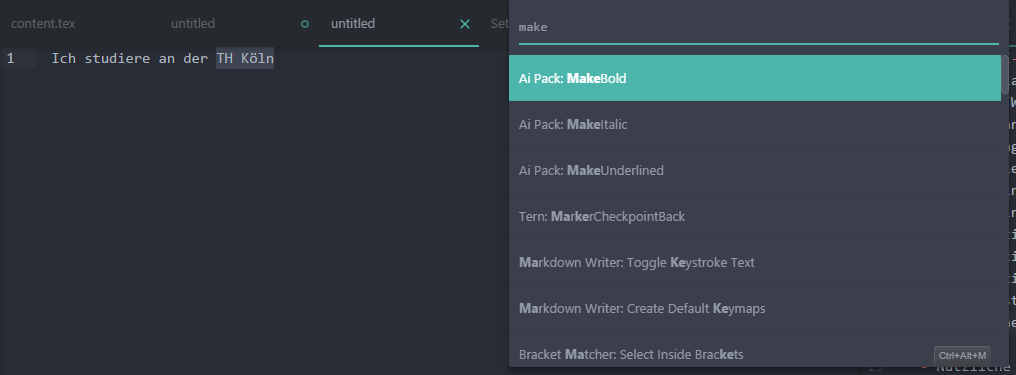
\includegraphics[scale=1.0]{img/make_bold_example.png}
                \caption{Konvertierung von markiertem Text}
            \end{minipage}
            \begin{tabular}{ | c | c | }
              \hline
              fetter Text & \texttt{\\textbf{fetter Text}} \\
              kursiver Text & \texttt{\\textit{kursiver Text}} \\
              unterstrichener Text & \texttt{\\underline{unterstrichener Text}} \\
              \hline
            \end{tabular}
            TODO: screenshots
        \subsection{Nutzung von Snippets über die Command Palette}
            TODO: screenshots

    \section{Entscheidung für die Entwicklung mit JavaScript}
    \textbf{Weglassen falls genug Content.}

    \section{Aufbau eines Atom Packages}
    \begin{figure}
        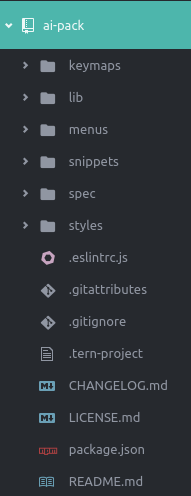
\includegraphics[scale=1.0]{img/package_structure.png}
        \caption{Atom Package Struktur}
    \end{figure}
    Wird eine neues Package im Atom Editor angeleget, wird die in Abbildung \textit{Atom Package Struktur} gezeigte Verzeichnis- und Dateistruktur angelegt. Ausgenommen der Konfigurationsdateien \texttt{.eslintrrc.js, .gitattributes, .gitignore, .tern-project}, welche nachträglich hinzugefügt worden sind und die Entwicklung des Packages erleichtern.

    Die für das RookieTeX Package wichtigsten Verzeichnisse sind \texttt{lib} und \texttt{snippets}. Im Verzeichnis \texttt{lib} befindet sich die Logik des Packages bestehend aus den Dateien:
    \begin{tabular}{ | c | c | }
      \hline
      \texttt{ai-pack-view.coffee} & Einstiegpunkt des Packages \\
      \hline
      \texttt{ai-pack.js} & Deklaration von Command Palette Befehlen und Package Einstellungen \\
      \hline
      \texttt{converter.js} & Funktionen zur Konvertierung von Text in TeX \\
      \hline
      \texttt{generator.js} & Funktionen zur Generieung eines TeX Projekts \\
      \hline
      \texttt{templates.js} & Funktionen zur Generierung von TeX Elementen \\
      \hline
      \texttt{utils.js} & Hilfsfunktionen \\
      \hline
    \end{tabular}

    Im Verzeichnis \texttt{snippets} befindet sich auschließlich die Datei \texttt{latex-snippets.cson}. Diese Datei im CoffeeScript Object Notation Format beinhaltet jegliche Snippets des Package, im Fall von RookieTeX also LaTeX Snippets. Die Snippets haben folgende Form:
    \insertcode{src/example_snippet.cson}{LaTeX Snippet Beispiel (LaTeX Tabelle)}

\chapter{Aufbau eines TeX Projekts}
    \section{Modulare Struktur eines TeX Projekts}
    Um die Erstellung eines TeX Projekts zu erleichtern, bietet es sich an eine modulare Struktur, also einen bestimmten Aufbau des Projekts zu nutzen. Es ist sinnvoll Dinge mit unterschiedlicher Semantik voneinander zu trennen. Zum Beispiel sollte sich ein Deckblatt oder ein Glossar nicht in der selben \texttt{.tex} Datei befinden wie der eigentliche Inhalt des im Projekt behandelten Themas. Des Weiteren sollten Projketübergreifende Einstellungen wie genutzte LaTeX Packages oder Seitenabstände in einer \texttt{.sty} Datei zusammengefasst sein. Diese Vorgehensweise hat den Vorteil das besonders in umfangreichen Projekten die Übersicht gewährleistet wird. In den \texttt{.tex} Dateien die den eigentlichen Inhalt des zu erstellenden Dokuments beinhalten, kann sich so hauptsächlich auf das schreiben von Text konzentriert werden.

    TeX liefert verschiedene Möglichkeiten zum auslagern und modularisieren von TeX-Komponenten. Als Basisfunktion kann der LaTeX-Befehl \texttt{\\include} gennant werden, welcher dazu dient verschiedene \texttt{.tex} Dateien in einer Datei zusammenzuführen. Der LaTeX-Compiler sorgt dann automatisch dafür, dass alle \texttt{.tex} Dateien in der angegebenen Reihenfolge kompiliert werden. Diese Funktionalität arbeitet sowohl auf einer Verzeichnisebene, als auch Verzeichnisübergreifend.

\chapter{Implementierung}
    \section{Implementierung der Generieung eines LaTeX-Projekts}
        TODO: Erklärung
    \section{Implementierung der Konvertierung von Plain Text Listen}
        TODO: Erklärung
    \section{Implementierung der Formatierung von Text}
        TODO: Erklärung
    \section{Implementierung der Nutzung von Snippets über die Command Palette}
        TODO: Erklärung
